\documentclass[12pt]{article}
\usepackage{setspace,graphicx,amsmath,geometry,fontspec,titlesec,soul,bm,subfigure}
\titleformat{\section}[block]{\LARGE\bfseries}{\arabic{section}}{1em}{}[]
\titleformat{\subsection}[block]{\Large\bfseries\mdseries}{\arabic{section}.\arabic{subsection}}{1em}{}[]
\titleformat{\subsubsection}[block]{\normalsize\bfseries}{\arabic{subsection}-\alph{subsubsection}}{1em}{}[]
\titleformat{\paragraph}[block]{\small\bfseries}{[\arabic{paragraph}]}{1em}{}[]
\setmainfont{Times New Roman}
\renewcommand{\baselinestretch}{1.15}
\geometry{a4paper,left=2.5cm,right=2.5cm,top=2.5cm,bottom=2.5cm}
\begin{document}
	\newpagestyle{main}{            
		\sethead{Ziqing Yu}{Bildverarbeitung 4}{3218051}     
		\setfoot{}{\thepage}{}
		\headrule
		\footrule
			}
	\pagestyle{main}
\section{Einleitung}
In dieser Übung werden 2 Projektive Bildtransformation durch homogene Koordinaten gemacht, 1 mal für eine Gebäudefassade und 1 mal für Seminarraum. 
\section{Punkte wählen}
Zunächst sind zumindest 4 identische Punkte auf jeweils Bilde zu wählen, hier sind 5 Punkten gewählt. Die gewählte Punkte sollen möglichst in einer Ebene sein:
\begin{figure*}[ht]\centering
	\subfigure[gewählte Punkte auf Bild 1]{
		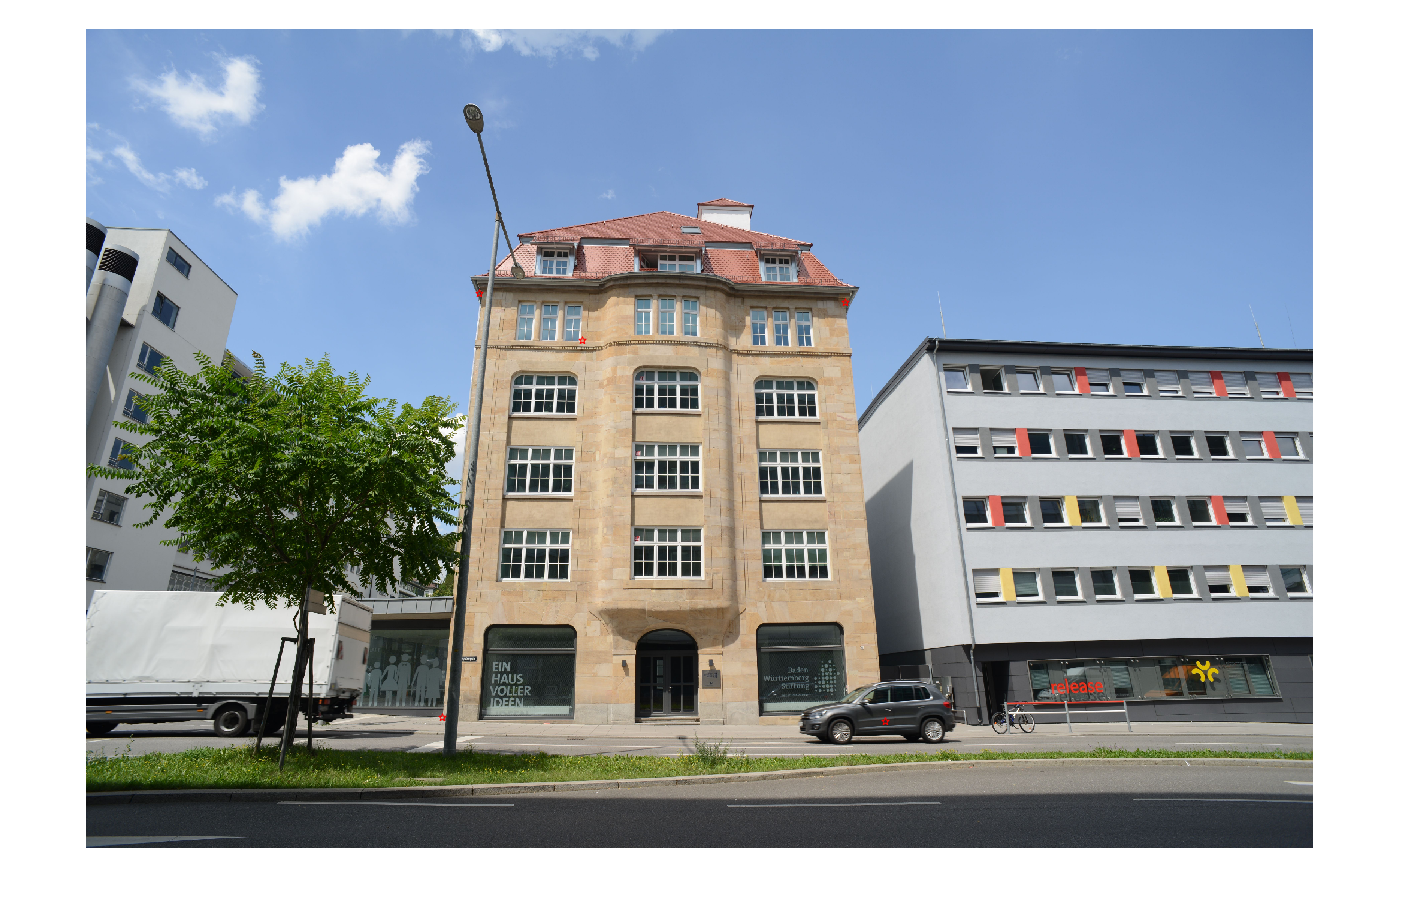
\includegraphics[width=0.45\textwidth]{P3.png}}
	\subfigure[gewählte Punkte auf Bild 2]{
		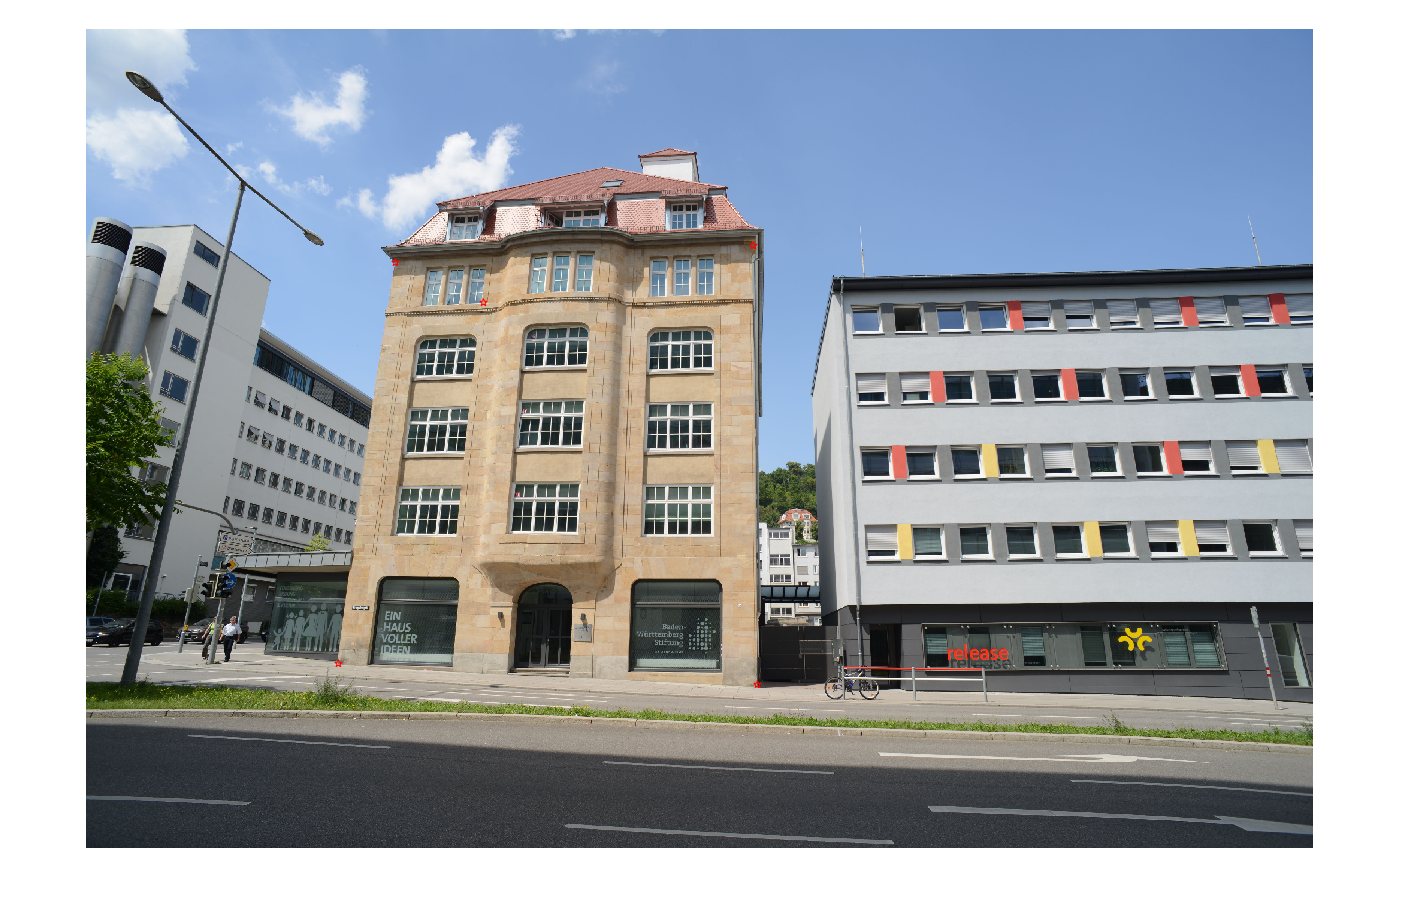
\includegraphics[width=0.45\textwidth]{P4.png}}
\end{figure*}
\begin{figure*}[ht]\centering
	\subfigure[Originalbilder mit gewählten Punkten]{
		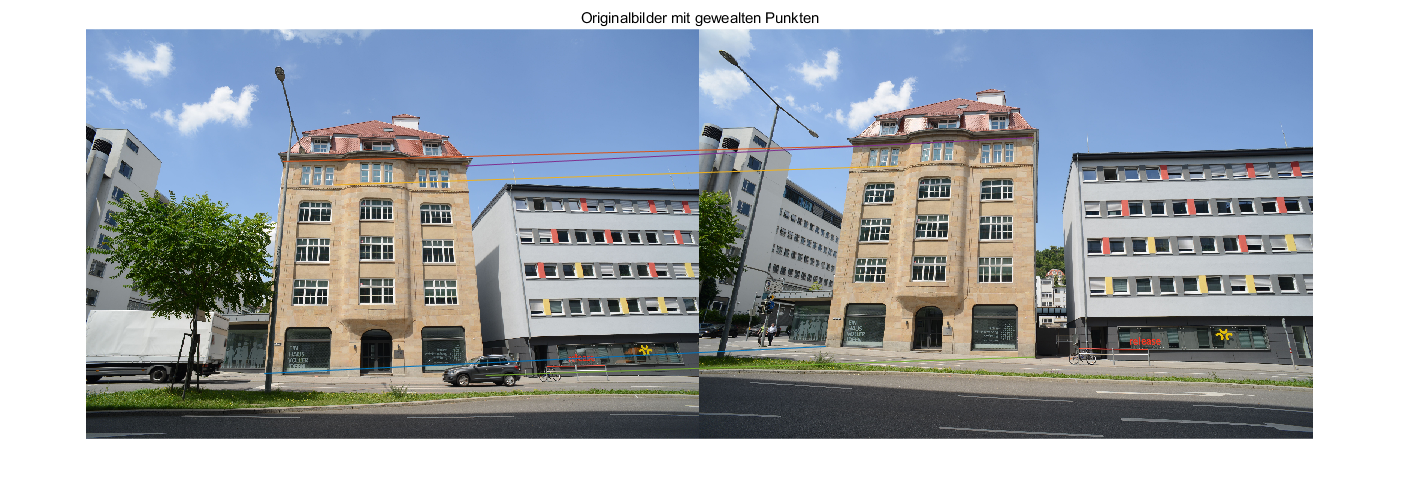
\includegraphics[width=0.9\textwidth]{identisch2.png}}
\end{figure*}
\noindent Um die Rechnung zu vereinfachen, werden die Koordinaten von identischen Punkten in Homogene Koordinate erweitert. Hier machen wir die zusätzliche Komponente $w=1$, also nutzen wir die normalisierte homogene Koordinaten.
\begin{equation*}
\begin{bmatrix}
x\\
y\\
\end{bmatrix} = \begin{bmatrix}
x\\
y\\
1
\end{bmatrix}
\end{equation*}
Wir definieren die homogene Koordinaten von erstem Bild $\bm{x_i}$ und von zweitem Bild $\bm{x'_i}$
\begin{equation*}
\bm{x'_i} = \bm{H} \cdot \bm{x_i} \longrightarrow \bm{x'_i} \times \bm{H} \cdot \bm{x_i} = 0
\end{equation*}
$\bm{H}$ ist die Transformationmatrix:
\begin{equation*}
\bm{H} = \begin{bmatrix}
h_1 & h_2 & h_3\\
h_4 & h_5 & h_6\\
h_7 & h_8 & h_9\\
\end{bmatrix}
\end{equation*}
Wie können einen Folgende Vektor einbauen:
\begin{equation*}
\bm{h} = \begin{bmatrix}
\bm{h_1}\\
\bm{h_2}\\
\bm{h_3}
\end{bmatrix} = \begin{bmatrix}
\bm{H}(1,:)\\
\bm{H}(2,:)\\
\bm{H}(3,:)\\
\end{bmatrix} \longrightarrow \bm{H}\cdot \bm{x_i} = \begin{bmatrix}
\bm{h}^{1T}\bm{x_i}  \\
\bm{h}^{2T}\bm{x_i}  \\
\bm{h}^{3T}\bm{x_i}
\end{bmatrix}
\end{equation*}
Ausmultiplizieren des Kreuzprodukts:
\begin{equation*}
\bm{x'_i} \times \bm{H} \cdot \bm{x_i} = \begin{bmatrix}
y'_i \bm{h}^{3T}\bm{x_i} - w'_i \bm{h}^{2T}\bm{x_i} \\
w'_i \bm{h}^{1T}\bm{x_i} - x'_i \bm{h}^{3T}\bm{x_i} \\
x'_i \bm{h}^{2T}\bm{x_i} - y'_i \bm{h}^{1T}\bm{x_i}
\end{bmatrix} = 0
\end{equation*}
Danach haben wir diese Gleichung:
\begin{equation*}
\begin{bmatrix}
\bm{0}^T & -w'_i\bm{x_i}^T & y'_i\bm{x_i}^T \\
w'_i\bm{x_i}^T & \bm{0}^T & -x'_i\bm{x_i}^T \\
-y'_i\bm{x_i}^T & x'_i\bm{x_i}^T & \bm{0}^T 
\end{bmatrix} \begin{bmatrix}
\bm{h_1} \\
\bm{h_2} \\
\bm{h_3}
\end{bmatrix} = 0
\end{equation*}
Weil nur 1 und 2 Zeile von obigen Matrix sind linear unabhängig:
\begin{equation*}
\begin{bmatrix}
\bm{0}^T & -w'_i\bm{x_i}^T & y'_i\bm{x_i}^T \\
w'_i\bm{x_i}^T & \bm{0}^T & -x'_i\bm{x_i}^T \\
\end{bmatrix} \begin{bmatrix}
\bm{h_1} \\
\bm{h_2} \\
\bm{h_3}
\end{bmatrix} = 0 \longrightarrow \bm{A} \cdot \bm{h} = 0
\end{equation*}
Mit Singulärwertzerlegung von $\bm{A}$ kriegen wir $\bm{H}$ :
\begin{gather*}
\bm{A} = \bm{UD} \bm{V}^T \\
\bm{H} = reshape(\bm{V}(:,9),\ 3,\ 3)^T
\end{gather*}
Mit Matrix $H$ dürfen wir die Transformation machen, die Bildgeometrie wird durch eine Umbildung von Bildpunkten auf vorgegebene Positionen verändert, deswegen sind Interpolationsverfahren benötigt, um nach der geometrischen Transformation für die neu berechneten, i.allg. nicht ganzzahligen Pixelpositionen aus den umliegenden Werten neue Grauwerte zuzuweisen. In MATLAB ist es mit 'Interp2' gemacht. 
\begin{figure*}[ht]\centering
	\subfigure[Originalbild und Transformiertes Bild]{
		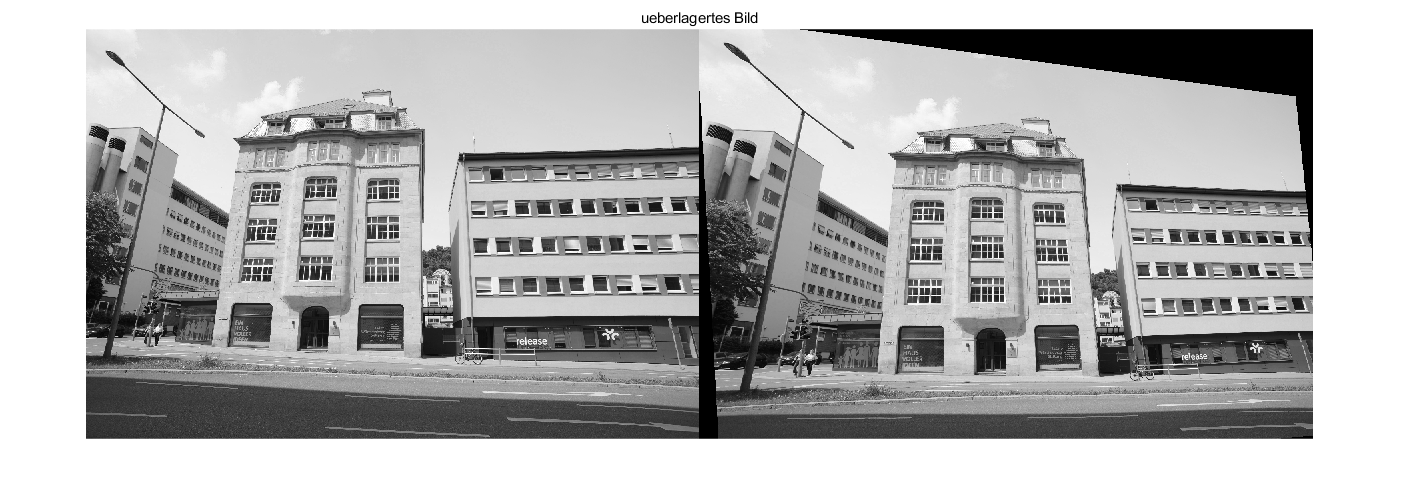
\includegraphics[width=0.9\textwidth]{transfor2.png}}
	\subfigure[Überlagertes Bild(Panoramabild)]{
		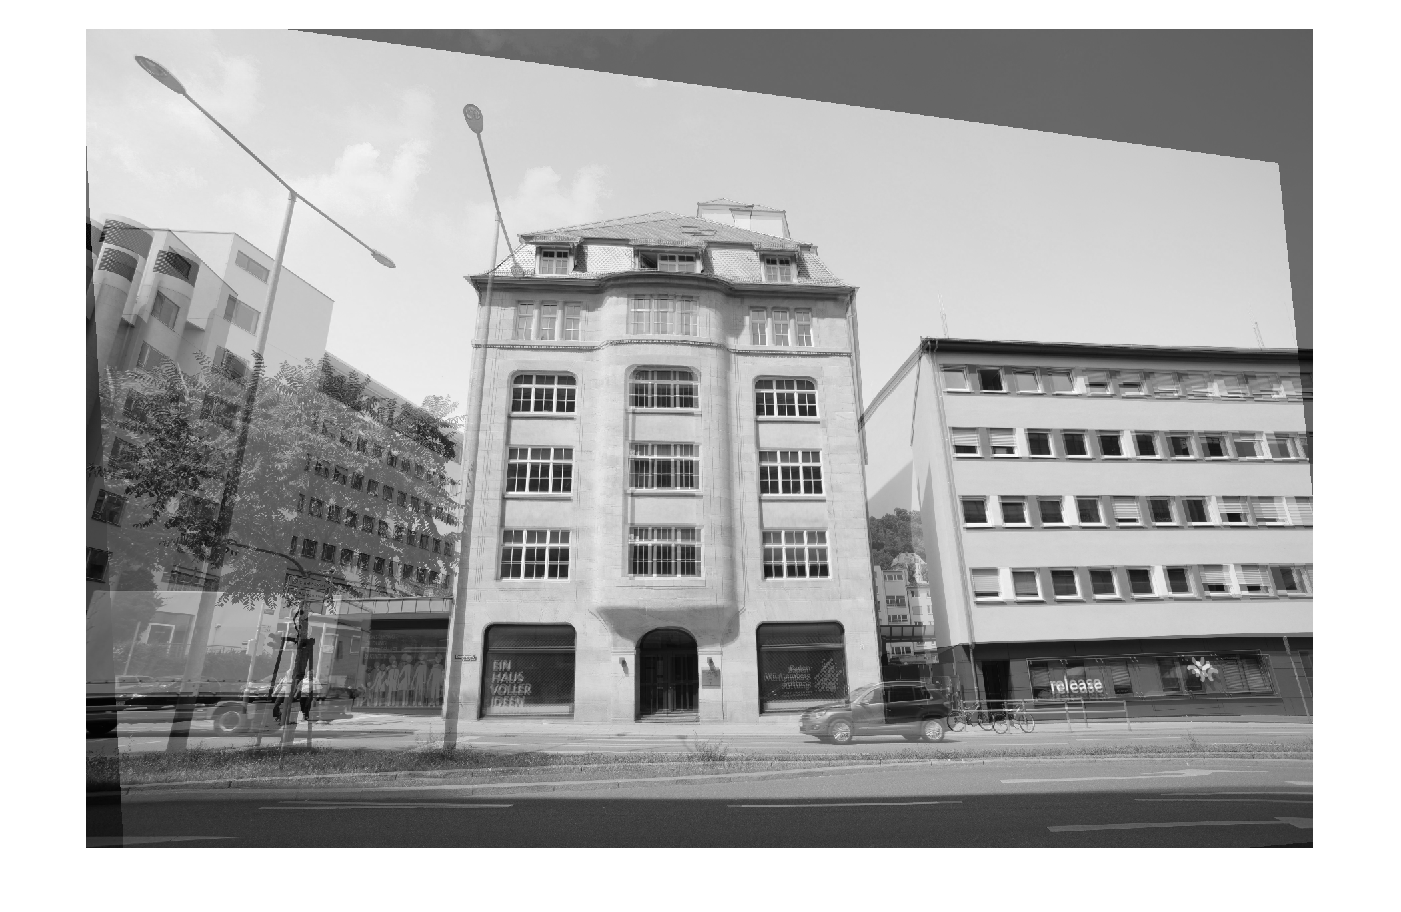
\includegraphics[width=0.9\textwidth]{ueberlar2.png}}
\end{figure*}
\newpage
Analog für die Seminarraumbilden.
\end{document}